\documentclass{article}\usepackage[]{graphicx}\usepackage[]{color}
%% maxwidth is the original width if it is less than linewidth
%% otherwise use linewidth (to make sure the graphics do not exceed the margin)
\makeatletter
\def\maxwidth{ %
  \ifdim\Gin@nat@width>\linewidth
    \linewidth
  \else
    \Gin@nat@width
  \fi
}
\makeatother

\definecolor{fgcolor}{rgb}{0.345, 0.345, 0.345}
\newcommand{\hlnum}[1]{\textcolor[rgb]{0.686,0.059,0.569}{#1}}%
\newcommand{\hlstr}[1]{\textcolor[rgb]{0.192,0.494,0.8}{#1}}%
\newcommand{\hlcom}[1]{\textcolor[rgb]{0.678,0.584,0.686}{\textit{#1}}}%
\newcommand{\hlopt}[1]{\textcolor[rgb]{0,0,0}{#1}}%
\newcommand{\hlstd}[1]{\textcolor[rgb]{0.345,0.345,0.345}{#1}}%
\newcommand{\hlkwa}[1]{\textcolor[rgb]{0.161,0.373,0.58}{\textbf{#1}}}%
\newcommand{\hlkwb}[1]{\textcolor[rgb]{0.69,0.353,0.396}{#1}}%
\newcommand{\hlkwc}[1]{\textcolor[rgb]{0.333,0.667,0.333}{#1}}%
\newcommand{\hlkwd}[1]{\textcolor[rgb]{0.737,0.353,0.396}{\textbf{#1}}}%
\let\hlipl\hlkwb

\usepackage{framed}
\makeatletter
\newenvironment{kframe}{%
 \def\at@end@of@kframe{}%
 \ifinner\ifhmode%
  \def\at@end@of@kframe{\end{minipage}}%
  \begin{minipage}{\columnwidth}%
 \fi\fi%
 \def\FrameCommand##1{\hskip\@totalleftmargin \hskip-\fboxsep
 \colorbox{shadecolor}{##1}\hskip-\fboxsep
     % There is no \\@totalrightmargin, so:
     \hskip-\linewidth \hskip-\@totalleftmargin \hskip\columnwidth}%
 \MakeFramed {\advance\hsize-\width
   \@totalleftmargin\z@ \linewidth\hsize
   \@setminipage}}%
 {\par\unskip\endMakeFramed%
 \at@end@of@kframe}
\makeatother

\definecolor{shadecolor}{rgb}{.97, .97, .97}
\definecolor{messagecolor}{rgb}{0, 0, 0}
\definecolor{warningcolor}{rgb}{1, 0, 1}
\definecolor{errorcolor}{rgb}{1, 0, 0}
\newenvironment{knitrout}{}{} % an empty environment to be redefined in TeX

\usepackage{alltt}

\title{How to Export Files for Sakai}
\IfFileExists{upquote.sty}{\usepackage{upquote}}{}
\begin{document}
\maketitle

\section{Text to Introduce your Blog}

For each blog, we'll need a introductory link -- text that encourages a reader to look at your blog from the introduction that I have outline. Crate a file called 'hook' and put some text in there that can be used in the introduction and I'll create a link to your blog. 

When submiting to the Sakai site, please include the 'hook' in the exported files.  

\section{Cleaning up Directory}

\begin{figure}
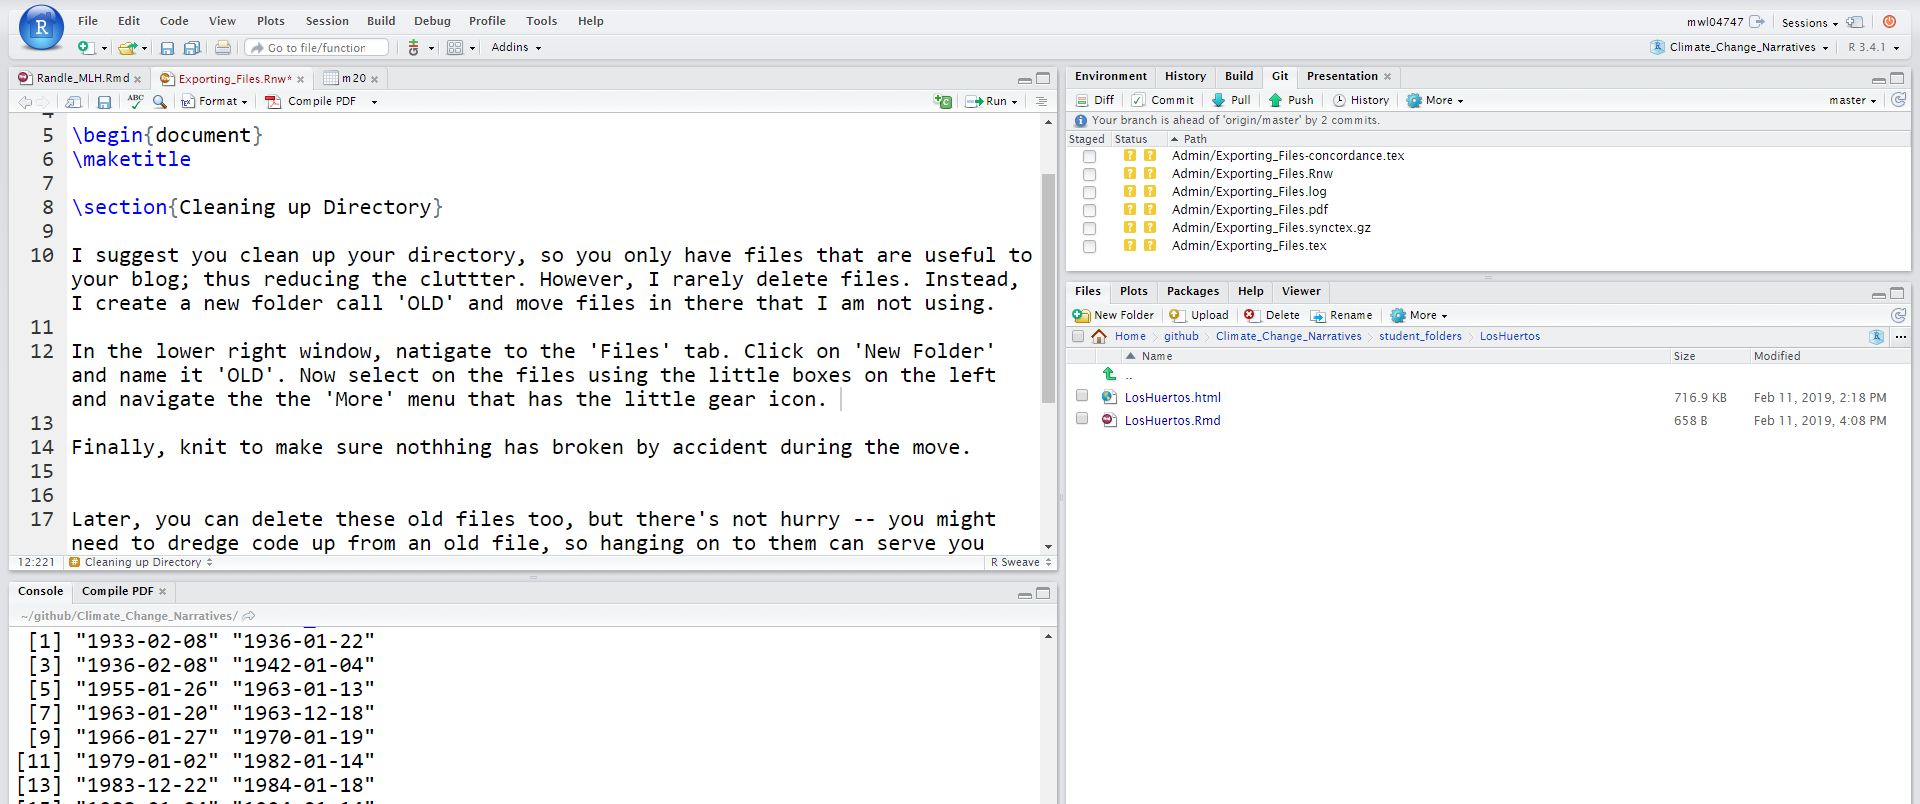
\includegraphics[width=\textwidth]{FourWindows}
\end{figure}

I suggest you clean up your directory, so you only have files that are useful to your blog; thus reducing the cluttter. However, I rarely delete files. Instead, I create a new folder call 'OLD' and move files in there that I am not using.

\begin{figure}
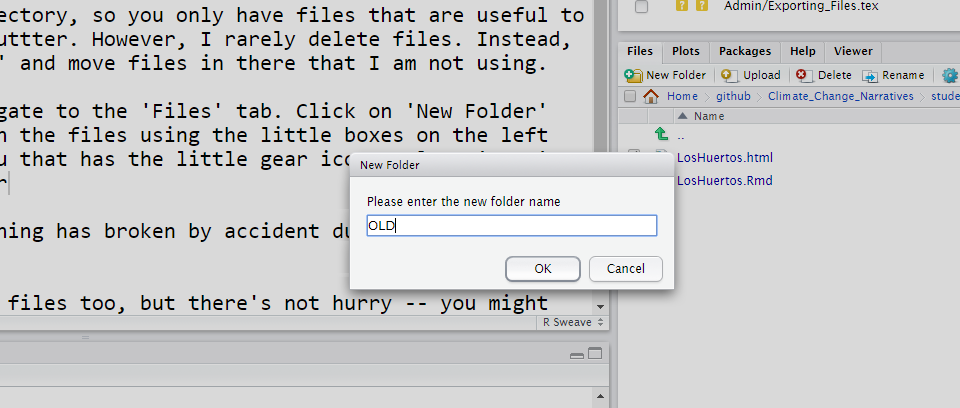
\includegraphics[width=\textwidth]{CreateFolder}
\end{figure}

In the lower right window, natigate to the 'Files' tab. Click on 'New Folder' and name it 'OLD'. Now select on the files using the little boxes on the left and navigate the the 'More' menu that has the little gear icon. Select 'Move' and choose the 'OLD' to move the files. Finally, knit to make sure nothhing has broken by accident during the move. 

\begin{figure}
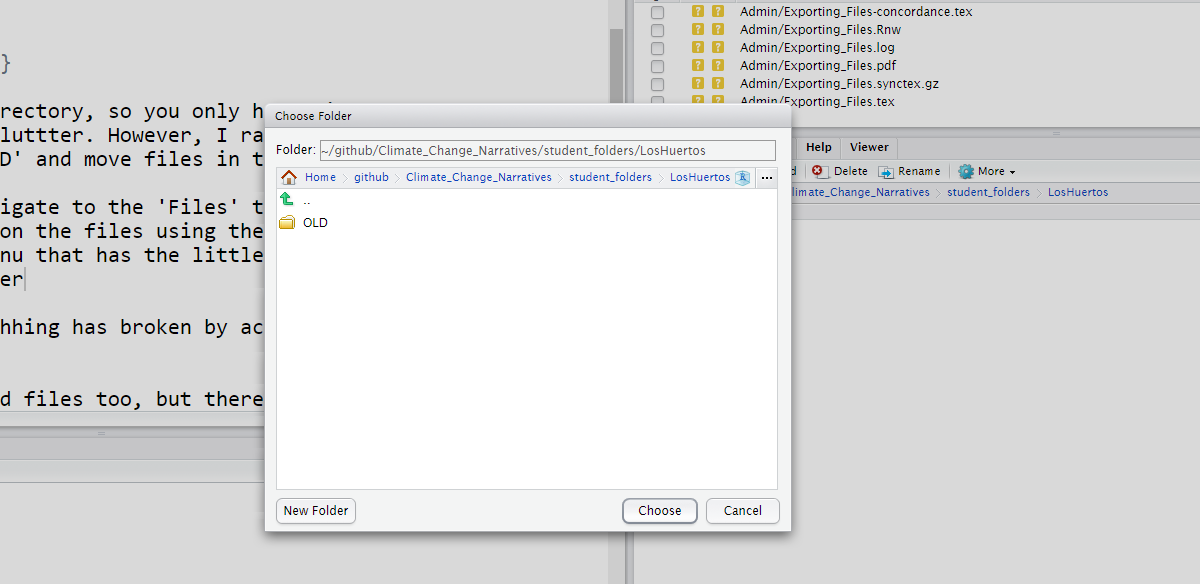
\includegraphics[width=\textwidth]{MoveFiles}
\end{figure}


Later, you can delete these old files too, but there's not hurry -- you might need to dredge code up from an old file, so hanging on to them can serve you later. 

\section{Exporting Files}

Similar to the moving process, you will select the files you want to export by checking the boxes on the left of the files and then navigate to the 'More' menu item with the gear icon. Then select export and R studio will prompt you to determine the location you want to download the file.

\begin{figure}[h]
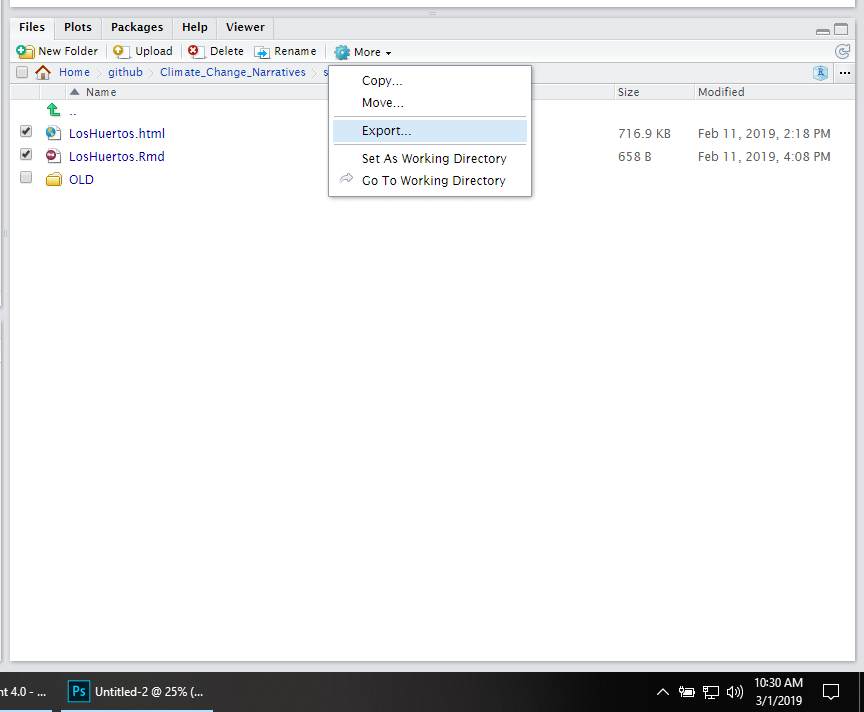
\includegraphics[width=\textwidth]{ExportFiles}
\end{figure}


Note: For PC users this is a zip file that can be uploaded directly to Sakai. However, for MAC users, you must compress the file so that it can be put into Sakai. 

I will then upload the files into the 'docs' directory, where I will knit the files to create the html. These files will by synced and publicly visible in about 10-15 minutes after I upload them. 


\end{document}
